\documentclass{beamer}
\usetheme{default}

\usepackage{graphicx}
\usepackage{amsmath}
\usepackage{amsthm}

\setbeamercolor{block title}{bg=blue!20, fg=black}
\setbeamercolor{block body}{bg=blue!5, fg=black}

\title{Elementary Column Matrices and the Smith Normal Form}
\author{Ethan Kalika and Chloe Borentain}
\date{December 2024}
\begin{document}

\begin{frame}
    \titlepage
\end{frame}
\begin{frame}{Linear Algebra Review}
    \begin{itemize}
        \item Given an $m \times n$ matrix $A$ there are three types of \textbf{elementary row operations}.
        \begin{itemize}
            \item \textbf{Adding a multiple of a row}, that is adding $c$ times row $i$ to row $j$.
            \item \textbf{Swapping 2 rows}, that is putting row $i$ in the position of row $j$ and $j$ in the position of $i$.
            \item \textbf{Scaling a row}, that is multiplying each entry in a row by some scalar $c$.
        \end{itemize}
    \end{itemize}
\end{frame}
\begin{frame}{Unimodular Elementary Row Operations}
    \begin{itemize}
        \item The 3 unimodular elementary row operations are almost exactly the same as the same as the elementary row operations except we can only add integral multiples or rows and for the third operation we are only allowed to scale by -1.
        \item The \textbf{unimodular elementary row operations} defined are as follows.
        \begin{itemize}
            \item \textbf{Adding a multiple of a row}, that is adding $c$ times row $i$ to row $j$ where $c \in \mathbb{Z}$.
            \item \textbf{Swapping 2 rows}, that is putting row $i$ in the position of row $j$ and $j$ in the position of $i$.
            \item \textbf{Scaling a row}, that is multiplying each entry in a row by some scalar -1.
        \end{itemize}
    \end{itemize}
\end{frame}
\begin{frame}{Matrix Representation}
    \begin{itemize}
        \item We can express the unimodular elementary row operations as left multiplication by elementary matrices.
        \item Given an $m \times n$ matrix $A$ and an integer $t$ we make the following notations.
        \begin{itemize}
            \item We will denote the elementary matrix corresponding to adding $t$ times row $j$ to row $i$ by $\rho_1(m, i, j, t)$.
            \item We will denote the elementary matrix corresponding to swapping rows $i$ and $j$ by $\rho_2(m, i, j)$.
            \item We will denote the elementary matrix corresponding to multiplying row $i$ by -1 as $\rho_3(m, i)$.
        \end{itemize}
    \end{itemize}
\end{frame}
\begin{frame}{Matrix Representation Continued}
    \begin{itemize}
        \item We define $\rho_1(m, i, j, t)$, $\rho_2(m, i, j)$, and $\rho_3(m, i)$ as follows.
        \begin{itemize}
            \item $\rho_1(m, i, j, t)_{ij} = t$.
            \item $\rho_2(m, i, j)_{ij} = \rho_2(m, i, j)_{ji} = 1$ and $\rho_2(m, i, j)_{ii} = \rho_2(m, i, j)_{jj} = 0$.
            \item $\rho_3(m, i)_{ii}$ = -1.
            \item All entries not explicitly defined are as they would be in $I_m$
        \end{itemize}
        \item Multiplying an $m \times n$ matrix $A$ on the left by one these matrices will perform the corresponding unimodular elementary row operation on $A$
    \end{itemize}
    \begin{figure}
            \centering
            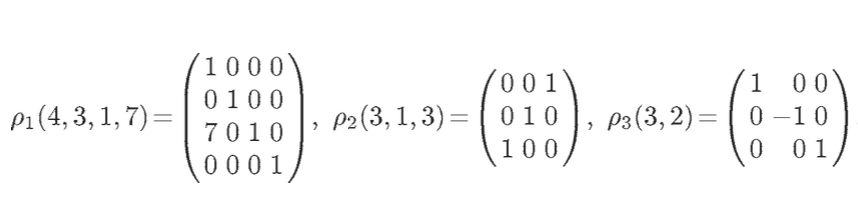
\includegraphics[width=0.8\textwidth]{UnimodularElementaryRowOperationsExample.png}
            \caption{Here are some examples of what such matrices may look like. \cite{holt2005handbook}}
        \end{figure}
\end{frame}
\begin{frame}{Unimodular Elementary Column Operations}
    \begin{itemize}
        \item The \textbf{unimodular elementary column operations} are defined in an analogous way to the unimodular elementary row operations.
        \begin{itemize}
            \item \textbf{Adding a multiple of a column}, that is adding $c$ times row $i$ to row $j$ where $c \in \mathbb{Z}$.
            \item \textbf{Swapping 2 columns}, that is putting row $i$ in the position of row $j$ and $j$ in the position of $i$.
            \item \textbf{Scaling a column}, that is multiplying each entry in a row by some scalar -1.
        \end{itemize}
    \end{itemize}
\end{frame}
\begin{frame}{Matrix Representation}
    \begin{itemize}
        \item We can express the unimodular elementary column operations as right multiplication by elementary matrices.
        \item Given an $m \times n$ matrix $A$ and an integer $t$ we make the following notations.
        \begin{itemize}
            \item We will denote the elementary matrix corresponding to adding a $t$ times row $j$ to row $i$ by $\gamma_1(n, i, j, t)$.
            \item We will denote the elementary matrix corresponding to swapping rows $i$ and $j$ by $\gamma_2(n, i, j)$.
            \item We will denote the elementary matrix corresponding to multiplying row $i$ by -1 as $\gamma_3(n, i)$.
        \end{itemize}
    \end{itemize}
\end{frame}
\begin{frame}{Matrix Representation Continued}
    \begin{itemize}
        \item We define $\gamma_1(n, i, j, t)$, $\gamma_2(n, i, j)$, and $\gamma_3(n, i)$ as follows.
        \begin{itemize}
            \item $\gamma_1(n, i, j, t)_{ij} = t$.
            \item $\gamma_2(n, i, j)_{ij} = \gamma_2(n, i, j)_{ji} = 1$ and $\gamma_2(n, i, j)_{ii} = \gamma_2(n, i, j)_{jj} = 0$.
            \item $\gamma_3(n, i)_{ii}$ = -1.
            \item All entries not explicitly defined are as they would be in $I_n$
        \end{itemize}
        \item Multiplying an $m \times n$ matrix $A$ on the right by one these matrices will perform the corresponding unimodular elementary column operation on $A$
    \end{itemize}
\end{frame}
\begin{frame}{What is $GL(n, \mathbb{Z})$?}
    \begin{itemize}
        \item In the coming slides we will often refer to $GL(n, \mathbb{Z})$.
        \item It is important to note here that we typically define matrices in a ring on fields like $\mathbb{R}$ or $\mathbb{Z}_p$.
        \item $\mathbb{Z}$ is not a field, so we take $GL(n, \mathbb{Z})$ to mean the group generated by invertible $n \times n$ integral matrices whose inverses are also integral.
    \end{itemize}
\end{frame}
\begin{frame}{Smith Normal From}
    \begin{itemize}
        \item The integral $m \times n$ matrix $M$ is said to be in \textbf{Smith normal form (SNF)} if the following conditions hold.
        \begin{itemize}
            \item $M_{ij} = 0$ whenever $i \neq j$
            \item $M_{ii} \geq 0$ for $1 \leq i \leq$ min($m$, $n$)
            \item For $1 \leq i \leq$ min($m$, $n$) we have $M_{ii}|M_{i+1, i+1}$
        \end{itemize}
    \end{itemize}
\end{frame}
\begin{frame}{Existence and Uniqueness of SNF}
    \begin{Theorem}
        Let $M$ be any $n \times n$ matrix over $\mathbb{Z}$. Then we can put $M$ into SNF by applying a sequence of elementary unimodular row and column operations to $M$. Hence, there exists an $A \in GL(m, \mathbb{Z})$ and $B \in GL(n, \mathbb{Z})$ such that $AMB$ is in $SNF$.
    \end{Theorem}
    \begin{theorem}
        Let $M$ be an $m \times n$ matrix over $\mathbb{Z}$. If $AMB$ and $CMD$ are both in SMF, with $A, C \in GL(m, \mathbb{Z})$ and $B, D \in GL(n, \mathbb{Z})$, then $AMB = CMD$.
    \end{theorem}
\end{frame}
\begin{frame}{SNF Example}
    \begin{itemize}
        \item \cite{holt2005handbook} provides and algorithm for finding the SNF of a given matrix
        \begin{itemize}
            \item This algorithm also serves as an algorithmic proof of the existence theorem for the SNF.
        \end{itemize}
        \item The following illustrates a matrix and its corresponding SNF.
    \end{itemize}
    \begin{figure}
        \centering
        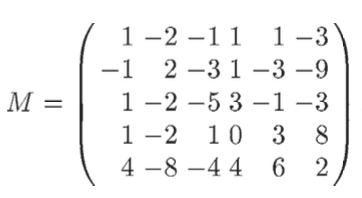
\includegraphics[width=0.5\textwidth]{SNFExample.png}
    \end{figure}
\end{frame}
\begin{frame}{SNF Example Continued}
    \begin{itemize}
        \item In the image below, $M$ is the SNF of the matrix on the previous slide and $AMB$ is equal to the matrix on the previous slide.
    \end{itemize}
    \begin{figure}
        \centering
        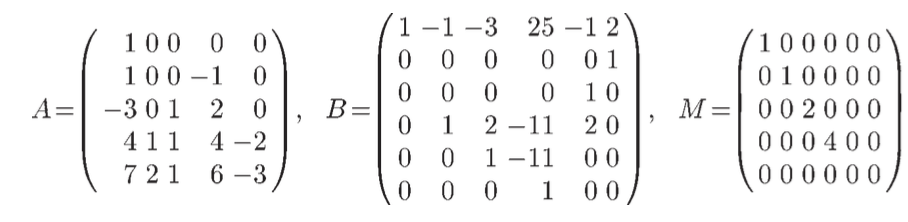
\includegraphics[width=0.75\textwidth]{Iter3.png}
    \end{figure}
    \begin{itemize}
        \item $M$ is in SNF because the only nonzero entries are on the diagonal and the divisibility condition for entries on the diagonal is also met.
    \end{itemize}
\end{frame}
\begin{frame}{How are Matrices Related to Group Theory}
    \begin{itemize}
        \item Any abelian group can be expressed as a direct sum of cycles.
        \item For example if we have $K := 2\mathbb{Z} \oplus 6\mathbb{Z} \oplus 12\mathbb{Z}$ and $G := \mathbb{Z}^3/K \cong \mathbb{Z}/2\mathbb{Z} \oplus \mathbb{Z}/6\mathbb{Z} \oplus \mathbb{Z}/12\mathbb{Z}$ then the elements of $K$ all lie in the row space of the matrix
        $$A = \begin{bmatrix}
            2 & 0 & 0\\
            0 & 6 & 0\\
            0 & 0 & 12\\
        \end{bmatrix}.$$
        \item $K$ however, is isomorphic to $\mathbb{Z}^3$ regardless of the coefficients of the cyclic groups, so while we can represent its elements as elements of a row space, it makes more sense to associate the matrix $A$ with $G$ because $G$ will vary depending on the coefficients in $K$.
        \item In fact performing modular elementary row operations on $K$ does not change its row space, so $G$ can be represented by any matrix derivable from $A$ by elementary row operations.
    \end{itemize}
\end{frame}
\begin{frame}{How is SNF related to Group Theory}
    \begin{itemize}
        \item Let the $m \times n$ matrix $M$ represent some cyclic group $K$.
        \begin{itemize}
            \item Note that the matrix representation can be rectangular if any coefficients in $K$ are 0. All such summands are moved to the end of the sum by convention.
        \end{itemize}
        \item Now let $A \in GL(m, \mathbb{Z})$ and $B \in GL(n, \mathbb{Z})$
        \item Notice that $AM$ is also an $m \times n$ matrix the rows of which are linearly independent linear combinations of rows of $M$. This means that $AM$ and $M$ have the same row space and hance both represent $\mathbb{Z}^n/K$.
    \end{itemize}
\end{frame}
\begin{frame}{How is SNF related to Group Theory Continued}
    \begin{itemize}
        \item Multiplying on the right by $B$ is the equivalent of performing column operations on $M$, which does change the row space. However, multiplication of vector representations of elements of $K$ by $B$ serves as an isomorphism of $K$ into some other group because multiplication by $B$ is an invertible linear transformation and so follows the homomorphism property.
        \item Because of this the abelian groups $\mathbb{Z}^n/K$ and $\mathbb{Z}^n/K'$, where $K$ and $K'$ represented by $M$ and $AMB$ respectively, are isomorphic.
        \item This is true in particular when $M = ANB$ where $N$ is the SMF of $M$.
    \end{itemize}
\end{frame}
\begin{frame}{The Divisibility Condition}
    \begin{itemize}
        \item An abelian group $G$ has type $(d_1,\ldots, d_n)$, for $d_i \in \mathbb{N}_0$ if it is isomorphic to the direct sum of cyclic groups $\mathbb{Z}/d_i\mathbb{Z}$. We say that $(d_1,\ldots, d_n)$ satisfies the \textbf{divisibility condition} if $d_i \neq 1$ for $1 \leq i \leq n$, and $d_i|d_{i+1}$ for $1 \leq i \leq n$.
    \end{itemize}
    \begin{Theorem}
        A finitely generated abelian group has type $(d_1,\ldots, d_n)$ for some $d_i \in \mathbb{N}_0$ that satisfy the divisibility criterion.
    \end{Theorem}
\end{frame}
\begin{frame}{Uniqueness of Type}
    \begin{Theorem}
        Suppose that the abelian group $G$ has type $(d_1,\ldots, d_n)$ and also has type $(c_1,\ldots, c_m)$, where $(d_1,\ldots, d_n)$ and $(c_1,\ldots, c_m)$ both satisfy the divisibility condition. Then $m = n$ and $d_i = c_i$ for $1 \leq i \leq n$.
    \end{Theorem}
    \begin{itemize}
        \item Note that the divisibility condition is necessary here because for example, the abelian groups of the types (4, 3, 5), (12, 5), (4, 15), (3, 20), and (60) are all isomorphic to each other, but have different number of factors.
    \end{itemize}
\end{frame}
\begin{frame}{Finding Abelian Invariants of $G/[G, G]$}
    \begin{itemize}
        \item The following example is from \cite{holt2005handbook}.
        \item The principal use of SNF in CTG is for finding invariants of $G/[G, G]$ in a finitely presented group $G$.
        \item We are given the following group presentation. (Relations without an ``=" sign are called relators are equal to 1 by convention).
    \end{itemize}
    \begin{figure}
        \centering
        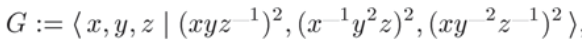
\includegraphics[width=0.75\textwidth]{Example.png}
    \end{figure}
    \begin{itemize}
        \item If we take $G/[G, G]$, then $x$, $y$, and $z$ become representatives of cosets that commute, so we can write the following.
    \end{itemize}
    \begin{figure}
        \centering
        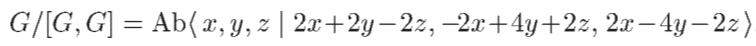
\includegraphics[width=0.75\textwidth]{AbelianizedRepresentation.png}
    \end{figure}
\end{frame}
\begin{frame}{Finding Abelian Invariants of $G/[G, G]$ Continued}
    \begin{itemize}
        \item We can represent $G/[G, G]$ by$$
        M = \begin{bmatrix}
            2 & 2 & -2\\
            -2 & 4 & 2\\
            2 & -4 & -2\\
        \end{bmatrix}
        $$ because $2x + 2y - 2z$, $-2x + 4y + 2z$, and $2x - 4y - 2z$ can all be treated as generators for cyclic subgroups of $\mathbb{Z}^3$ which can be added to create a subgroup, $K$ of $\mathbb{Z}^3$ and $G/[G, G] \cong \mathbb{Z}^n/K$.
        \item $M$ however, does not tell us much about $K$ and $G/[G, G]$ so we can bring it into SNF as shown below.
    \end{itemize}
    \begin{figure}
        \centering
        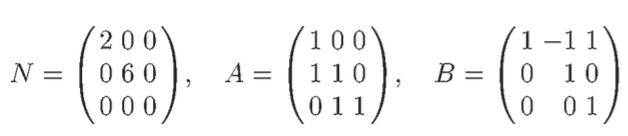
\includegraphics[width=0.75\textwidth]{SNF.png}
    \end{figure}
\end{frame}
\begin{frame}{Finding Abelian Invariants of $G/[G, G]$ Continued}
    \begin{itemize}
        \item From the SNF of $M$ we see that $G/[G, G] \cong H :=\mathbb{Z}/2\mathbb{Z} \oplus \mathbb{Z}/6\mathbb{Z} \oplus \mathbb{Z}$.
        \item The matrix $B$ also shows us the epimorphism, $\mu$ from $G/[G, G]$ to $H$.
        \item More specifically, it shows us that if $a$, $b$, and $c$ are taken to be the generators of $H$, then $\mu(x) = a - b + c$, $\mu(y) = b$, and $\mu(z) = c$.
    \end{itemize}
\end{frame}
\begin{frame}{References}
    \bibliographystyle{amsalpha}
    \bibliography{references}
\end{frame}
\end{document}